\documentclass[11pt,a4paper]{article}
\usepackage[utf8]{inputenc}
\usepackage[T1]{fontenc}
\usepackage{amsmath,amssymb}
\usepackage{graphicx}
\usepackage{booktabs}
\usepackage{hyperref}
\usepackage[margin=1in]{geometry}
\usepackage{float}

\title{SL-GPS Validation Report:\\GRI-Mech 3.0 Mechanism Reduction}
\author{SL-GPS Automated Validation}
\date{\today}

\begin{document}
\maketitle

\begin{abstract}
Validation of the SL-GPS method on GRI-Mech 3.0 (53 species, 325 reactions) for CH$_4$/air autoignition. Training data generated over T=900--2000~K, P=1--20~atm. Validated on 6 cases spanning the parameter space.
\end{abstract}

\section{Configuration}

\begin{table}[H]
\centering
\caption{Training parameters}
\begin{tabular}{lcc}
\toprule
Parameter & Min & Max \\
\midrule
Temperature & 900~K & 2000~K \\
Pressure & 1~atm & 20~atm \\
$X_{\text{CH}_4}$ & 0.02 & 0.10 \\
$X_{\text{O}_2}$ & 0.10 & 0.25 \\
$X_{\text{N}_2}$ & 0.60 & 0.80 \\
GPS $\alpha$ & \multicolumn{2}{c}{0.001} \\
Training cases & \multicolumn{2}{c}{20} \\
\bottomrule
\end{tabular}
\end{table}

\section{Validation Results}

\begin{figure}[H]
\centering
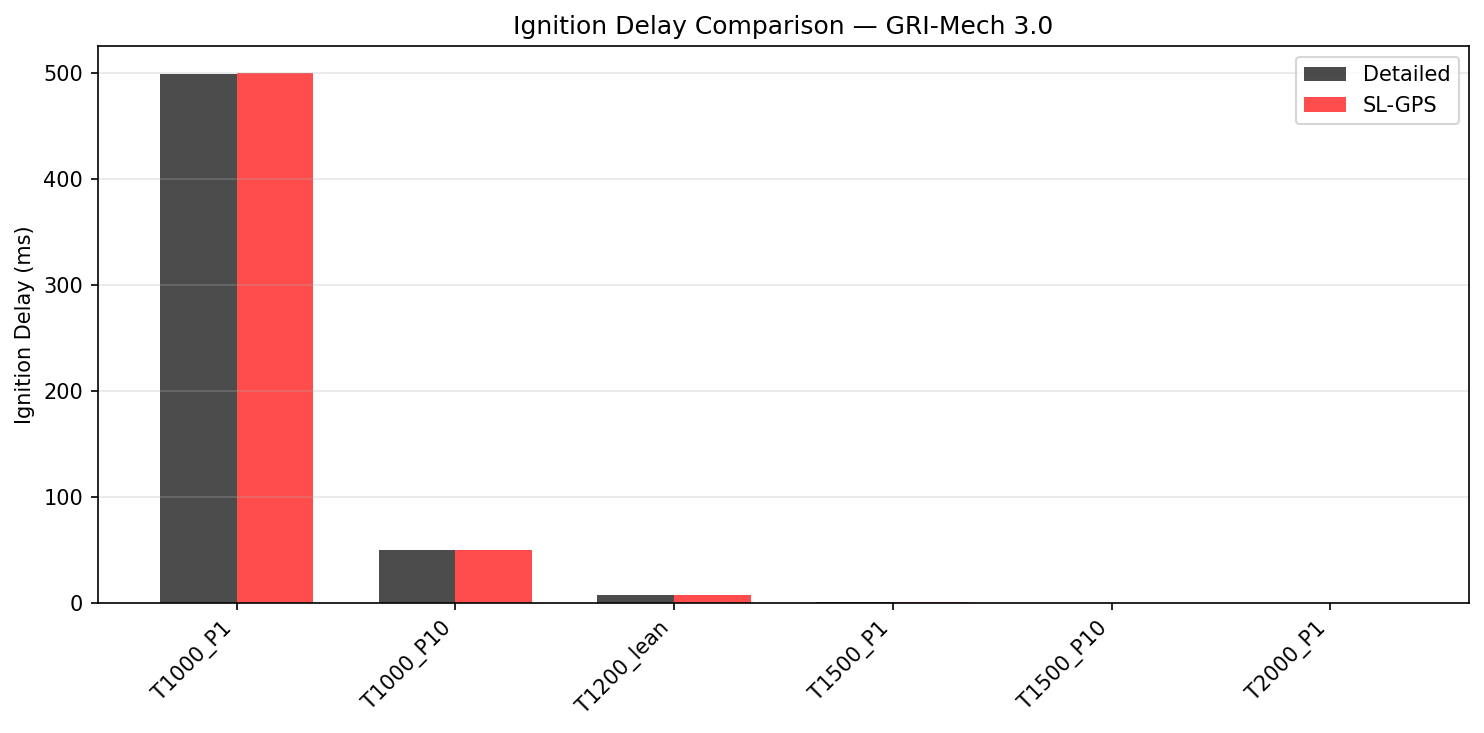
\includegraphics[width=0.9\textwidth]{results/ignition_delay_summary.png}
\caption{Ignition delay comparison: Detailed vs SL-GPS}
\end{figure}

\begin{figure}[H]
\centering
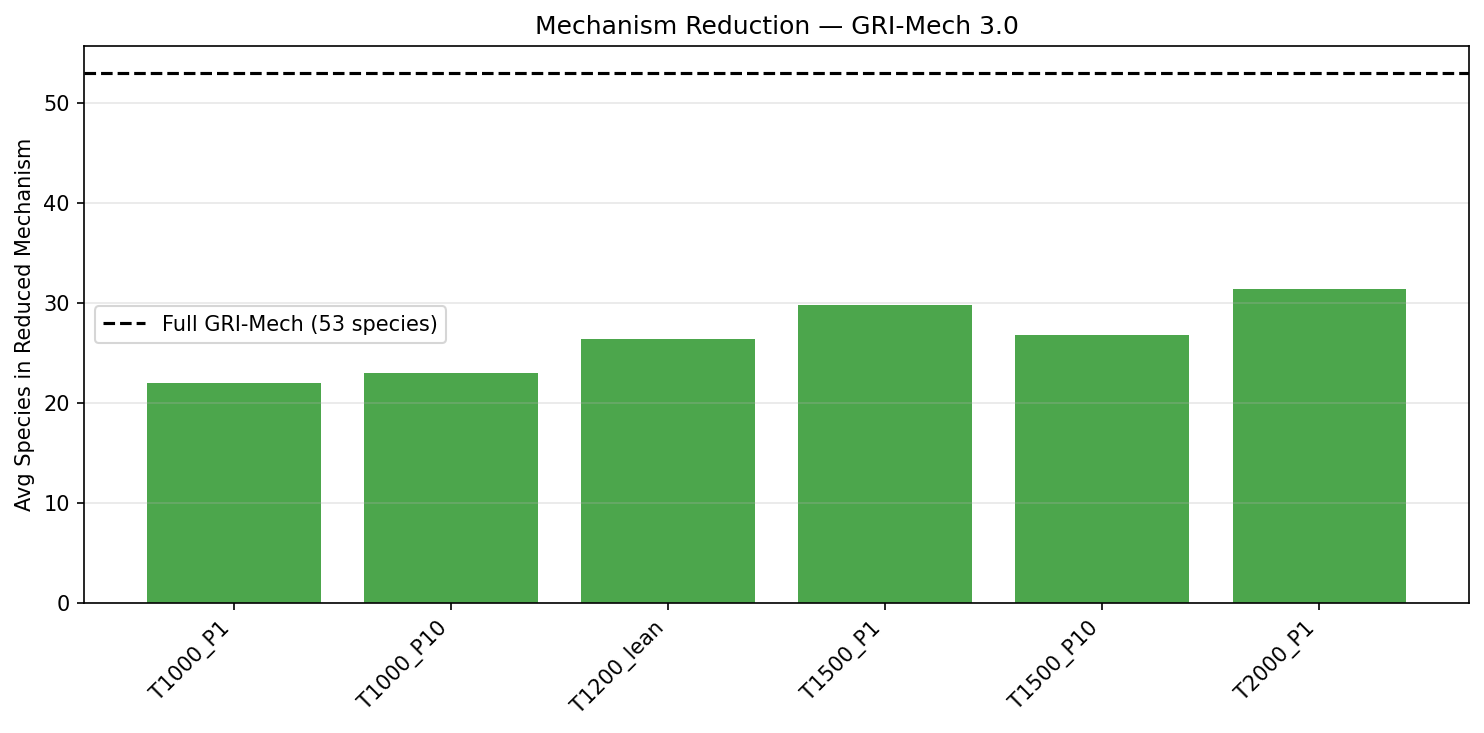
\includegraphics[width=0.9\textwidth]{results/reduction_summary.png}
\caption{Average species count in reduced mechanism per case}
\end{figure}

\begin{figure}[H]
\centering

\includegraphics[width=0.9\textwidth]{results/T1500_P1.png}
\caption{Case: T=1500K, P=1atm, $\phi$=1.0}
\end{figure}

\begin{figure}[H]
\centering

\includegraphics[width=0.9\textwidth]{results/T1500_P10.png}
\caption{Case: T=1500K, P=10atm, $\phi$=1.0}
\end{figure}

\begin{figure}[H]
\centering

\includegraphics[width=0.9\textwidth]{results/T2000_P1.png}
\caption{Case: T=2000K, P=1atm, $\phi$=1.0}
\end{figure}

\begin{figure}[H]
\centering
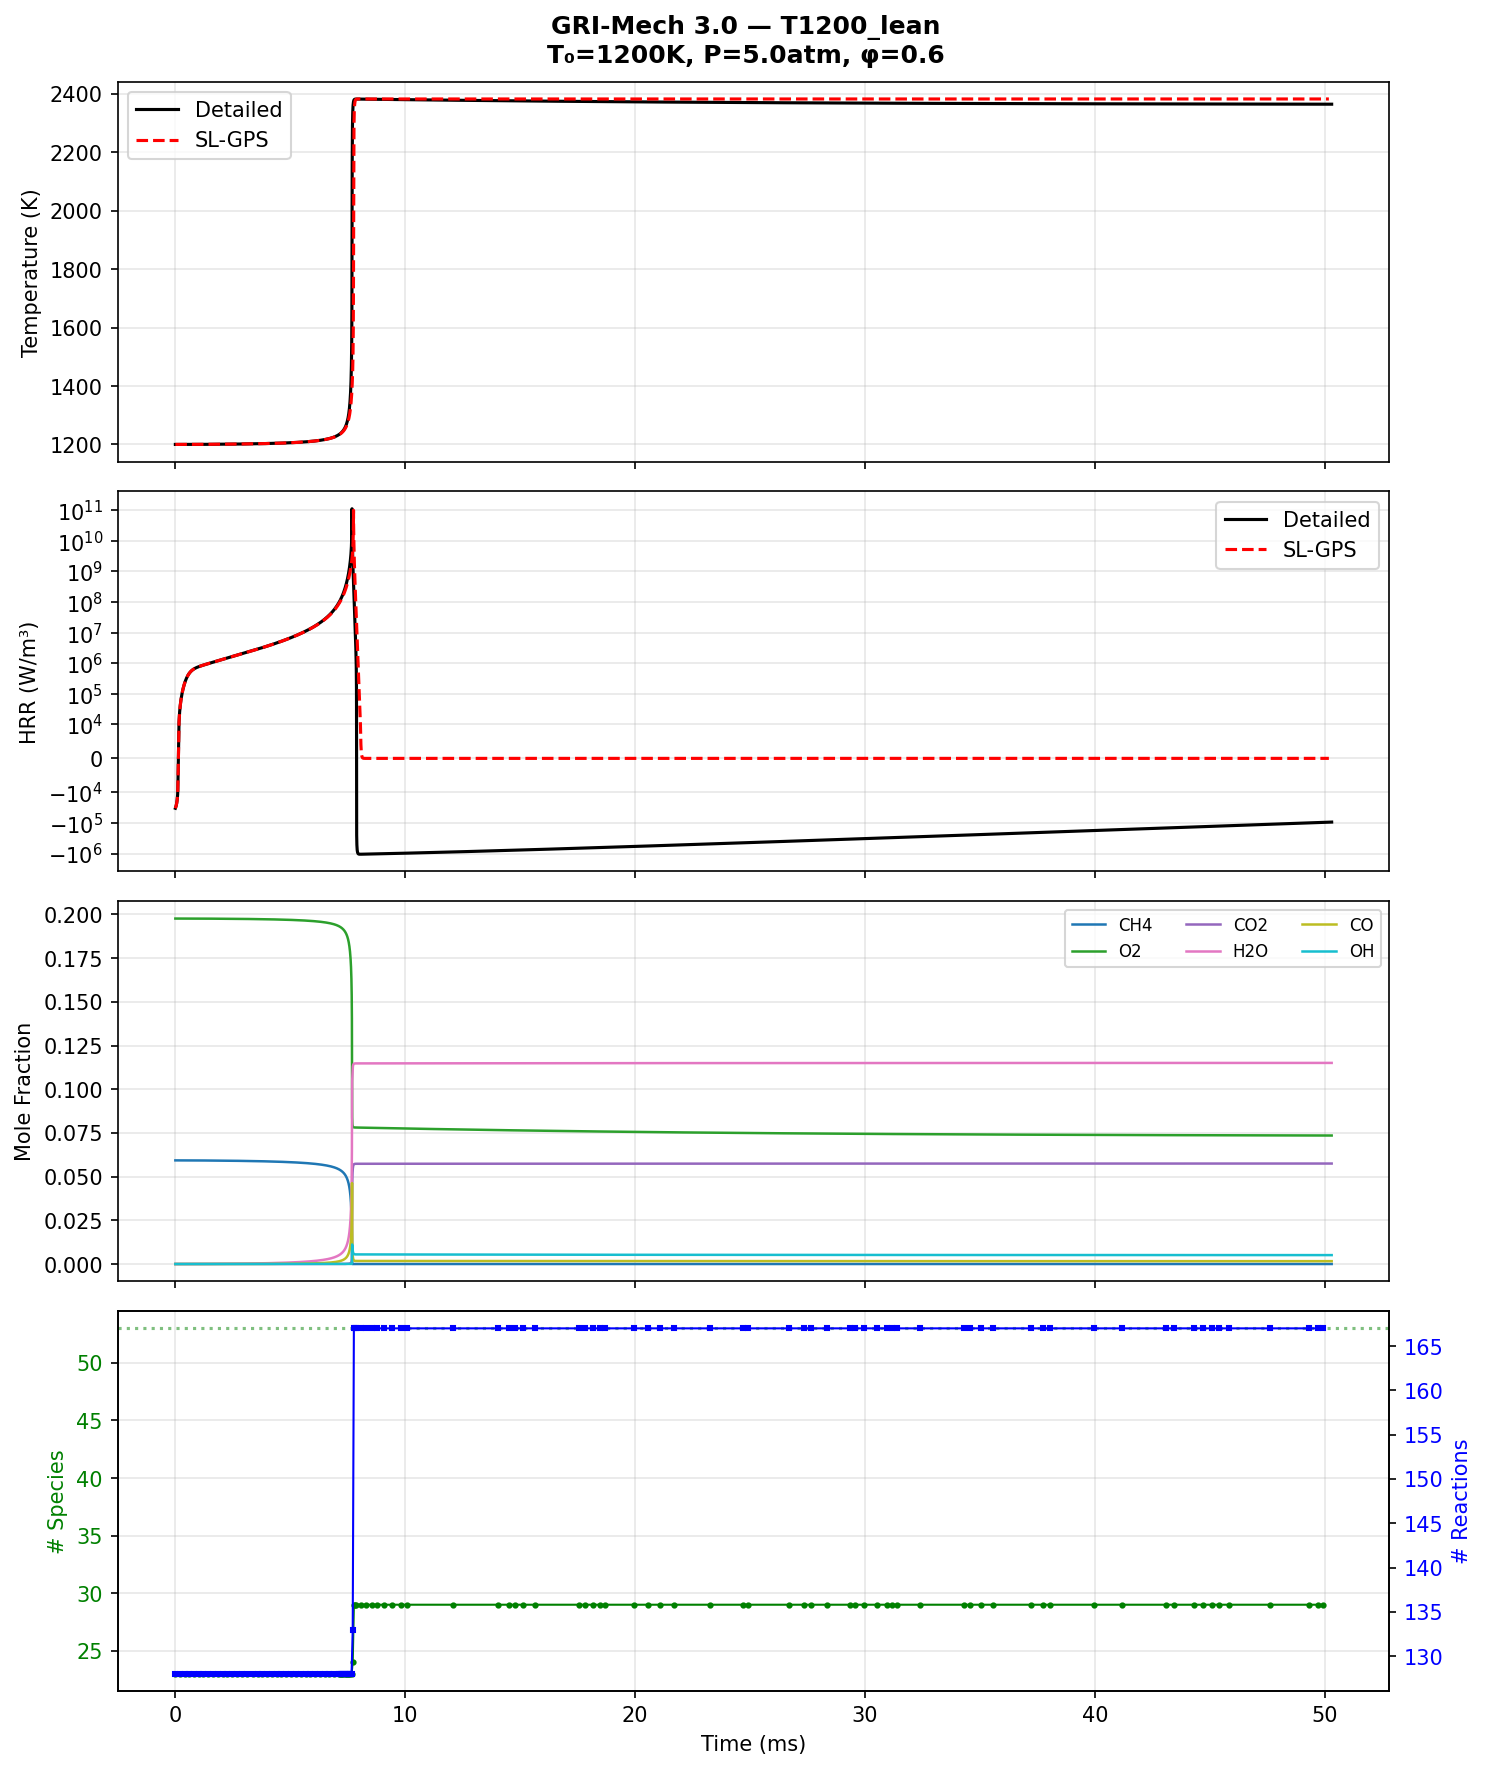
\includegraphics[width=0.9\textwidth]{results/T1200_lean.png}
\caption{Case: T=1200K, P=5atm, $\phi$=0.6 (lean)}
\end{figure}

\end{document}
